% !TeX spellcheck = en_US
% !TeX encoding = UTF-8
% !TeX program = xelatex
% Привет всем!

\documentclass[12pt]{article}
\usepackage[left=2cm, right=2cm, top=2cm, bottom=2cm]{geometry}
\usepackage{float}

\usepackage{bbm}
\usepackage{fontspec}
\usepackage{polyglossia} 
\usepackage{amsmath,amsfonts,amssymb,amsthm,mathtools}
\usepackage{amsmath}
\usepackage{stmaryrd}
\usepackage{bm}
\usepackage{graphicx}
\usepackage{subcaption}
\usepackage{bbm}
\usepackage{enumitem}
%\usepackage{enumerate}
\usepackage[bookmarks=false]{hyperref}

\usepackage{fancyvrb}

\usepackage{adjustbox}

% \usepackage{csquotes}
% \usepackage[backend=biber, style=apa, autocite=inline]{biblatex}
% \addbibresource{bibl.bib} 

% \usepackage{natbib}

\setsansfont{Linux Biolinum O}
\setromanfont{Linux Biolinum O} 
\setmonofont[Mapping=tex-text]{Courier New}

\usepackage{xcolor}
\usepackage{soul}

\setdefaultlanguage{english}

\newcommand{\N}{\mathbb{N}}
\newcommand{\Z}{\mathbb{Z}}
\newcommand{\E}{\mathbb{E}}
\DeclareMathOperator{\corr}{\mathop{corr}}
\DeclareMathOperator{\Corr}{\mathop{Corr}}
\DeclareMathOperator{\cov}{\mathop{cov}}
\DeclareMathOperator{\Cov}{\mathop{Cov}}
\DeclareMathOperator{\var}{\mathop{var}}
\DeclareMathOperator{\Var}{\mathop{Var}}
\DeclareMathOperator{\tr}{\mathop{tr}}
\DeclareMathOperator{\diag}{\mathop{diag}}
\DeclareMathOperator{\plim}{\mathop{plim}}
\DeclareMathOperator{\mmod}{\mathop{mod}}

\newcommand{\toD}{\stackrel{d}{\longrightarrow}}
\newcommand{\toP}{\stackrel{p}{\longrightarrow}}
\newcommand{\norm}[1]{\left\lVert#1\right\rVert}
\newcommand{\approxtext}[1]{\ensuremath{\stackrel{\text{#1}}{\sim}}}
\newcommand{\?}{\stackrel{?}{=}}
\renewcommand{\epsilon}{\varepsilon}
\renewcommand{\phi}{\varphi}

\mathtoolsset{showonlyrefs=true}

\usepackage{pgffor,newfile}
\newcommand*{\conoptprb}[4][\max]{%
    \newoutputstream{constraints}
    \openoutputfile{\jobname.constraints}{constraints}
    \foreach \entry [count=\ni] in {#4}
    {
        \ifnum\ni=1
            \addtostream{constraints}{& \text{  s.t.} & & \entry \\}
        \else
            \addtostream{constraints}{& & & \entry \\}
        \fi
    }
    \closeoutputstream{constraints}

  \begin{equation}
  \begin{aligned}
  & \underset{#2}{#1} & & #3 \\
  \input{\jobname.constraints}
  \end{aligned}
  \end{equation}
}


\begin{document}
\title{\vspace{-1.5cm} Advanced Topics in Macroeconomics 1. Problem Set 1}
\author{Evgenii Ivanov \and Walter Verwer}
\date{November 5, 2021}
 
\maketitle

\section*{Problem 1}

\subsection*{(a) Solve the model by value function iteration.}
Solving the model via value function iteration gives us the results displayed in figures \ref{fig:pol} and \ref{fig:val}.
\begin{figure}[htbp!]
    \centering
    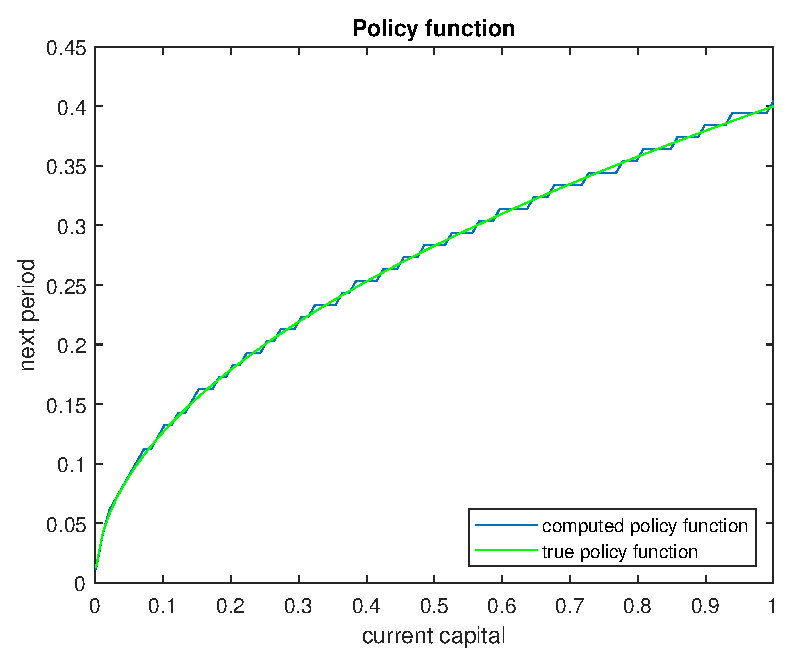
\includegraphics[width=0.45\textwidth]{PS1/1_Policy_Function_without.eps}
    \caption{Policy function using the brute-force method. Parameters: $\delta=1$, $\beta=0.96$, and $\alpha=0.3$.}
    \label{fig:pol}
\end{figure}

\begin{figure}[htbp!]
    \centering
    \includegraphics[width=0.45\textwidth]{PS1/1_Value_function_without.eps}
    \caption{Value function using the brute-force method. Parameters: $\delta=1$, $\beta=0.96$, and $\alpha=0.3$.}
    \label{fig:val}
\end{figure}

\begin{table}[htbp!]
    \centering
    \begin{tabular}{c|c|c}
         Method & Time (sec) & Number of iterations \\
         \hline
         Brute-force & 0.204910 & 395 \\
         Monotonicity & 0.186577 & 395 \\
         Concavity & 0.178771 & 395 \\
         Howard's pol. & 0.016517 & 18
    \end{tabular}
    \caption{Performance for the different methods. Parameters: $\delta=1$, $\beta=0.96$, and $\alpha=0.3$.}
    \label{tab:res}
\end{table}

\subsection*{(b) Exploit monotonicity of the policy function and evaluate its performance.}
In table \ref{tab:res} we have displayed the four different methods to compute the value function. We observe that exploiting monotonicity is faster than the brute-force method, but slower than exploiting concavity and Howard's method. The number of iterations is the same for all methods except the Howard's policy iteration method.

\subsection*{(c) Exploit concavity of the value function and evaluate its performance.}
Looking at table \ref{tab:res}, we see that concavity is the second fastest method. It ranks behind Howard's method and before the rest.

\subsection*{(d) Code Howard's policy iteration and evaluate its performance.}
Looking at table \ref{tab:res} again, we now observe a large increase in performance, compared to the other methods. Also, the number of iterations decreases significantly. As a side note, we used 30 iterations for updating the value function with Howard's method.




\section*{Problem 2}

Firstly let us derive the expression for the steady state level of capital.

The value function is:

\[
V(K) = \max_{k'} [ u(zf(k) + (1-\delta)k - k') + \beta V(k')]
\]

The first order condition:

\[
-u_c (c) + \beta V(k') = 0
\]
where $c = zf(k) + (1-\delta)k - k'$

The envelope condition:

\[
V'(k) = u_c (c) (zf'(k) + 1-\delta)
\]

Therefore if we combine them together we get the Euler equation:

\[
u_c (c) = \beta u_c (c') (zf'(k') + 1-\delta) 
\]

In the steady state $k'=k=k^*$ and $c$ is also constant:

\[
1 = \beta (zf'(k^*) + 1 - \delta)
\]
\[
f'(k^*) = z^{-1} \left( \frac{1}{\beta} - 1 + \delta \right)
\]

If we assume $f(k) = k^\alpha$ then $f'(k) = \alpha k^{\alpha-1}$ and then the steady state capital level is:

\[
k^* = \left[ \frac{1}{\alpha z} \left( \frac{1}{\beta} - 1 + \delta \right) \right]^{\frac{1}{\alpha-1}}
\]

\section*{Problem 3}
In figure \ref{fig:lin_int} one can see the results of the linear interpolation routine. It is not a very interesting graph, because the lines perfectly overlap. Details can be found in our code.

\begin{figure}[htbp!]
    \centering
    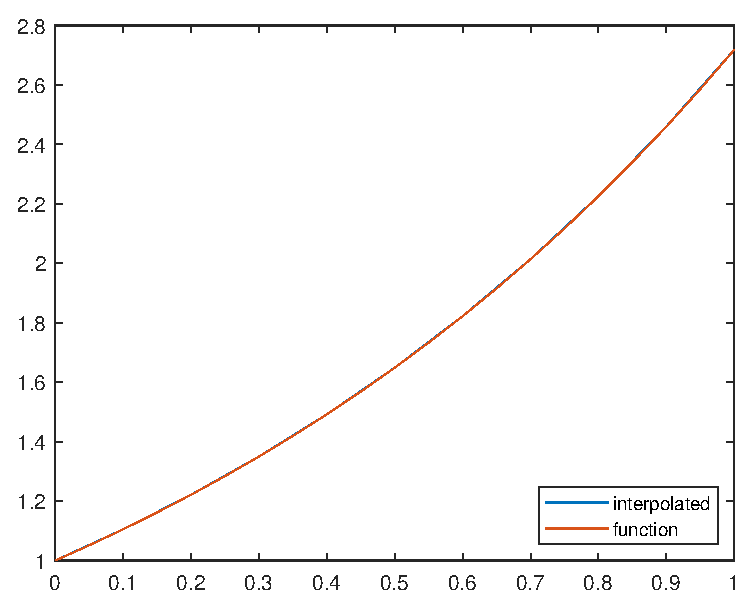
\includegraphics[width=0.45\textwidth]{PS1/ps3.eps}
    \caption{Result of linear interpolation routine.}
    \label{fig:lin_int}
\end{figure}


\section*{Problem 4}

In the bisection method, the error ($e$) is halved after every iteration ($n$): $\frac{e_{n+1}}{e_n} = \frac{1}{2}$. Thus, $e_{n+1} = \frac{e_n}{2}$. Hence, by definition the bisection method converges linearly at rate $\frac{1}{2}$.


\end{document}